%نام و نام خانوادگی:
%شماره دانشجویی: 
\مسئله{پارسر \lr{LALR(1)}}

\پاسخ{ }
\\
الف) عکس دیاگرام در زیر قرار داده شده است:
\graphicspath{{./images/}}
\begin{center}
	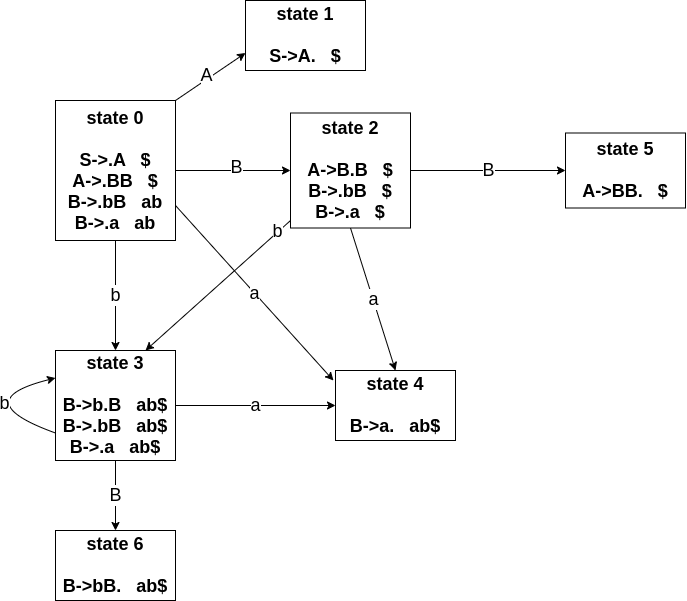
\includegraphics[scale=0.7]{compiler_hw2_q9.png}
\end{center}
عکس جدول در زیر قرار داده شده است:
\include{{./images}}
\begin{center}
	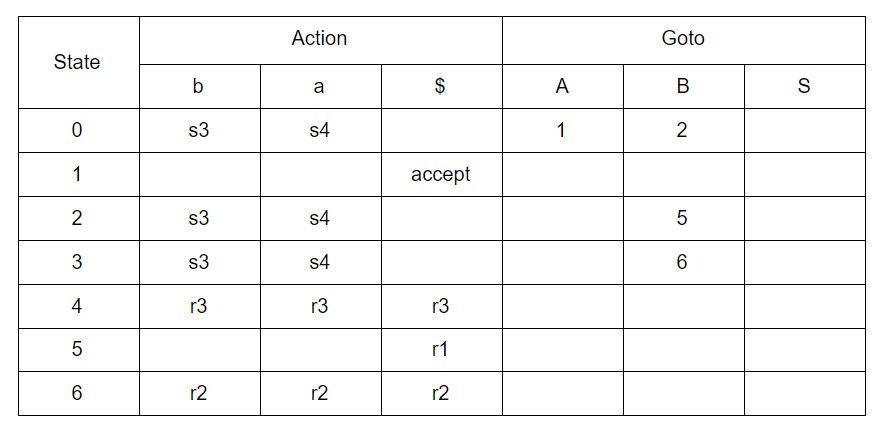
\includegraphics[scale=0.9]{compiler_hw2_q9_table.png}
\end{center}
ب) درخت پارس $babba$ را در پایین نوشته‌ایم: (دقت شود که حروفی که بین دو | می‌آیند در مرحله بعدی قرار است با هم، به کمک قاعده تولید reduce شوند)
\begin{latin}
	b
	\\
	b a
	\\
	b |a|
	\\
	b B
	\\
	|b B|
	\\
	B
	\\
	B b
	\\
	B b b
	\\
	B b b a
	\\
	B b b |a|
	\\
	B b b B
	\\
	B b |b B|
	\\
	B b B
	\\
	B |b B|
	\\
	B B
	\\
	|B B|
	\\
	A
\end{latin}
در نهایت درخت پارس رشته به صورت زیر می‌شود:
\begin{center}
	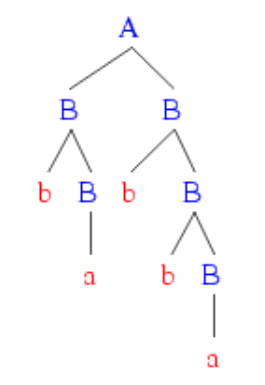
\includegraphics{babba.png}
\end{center}










